\chapter{Design}
\label{cha:development}

In this chapter, the design of the project will be described. Following some preliminary considerations, multiple iterations were developed in order to look for the best possible solution to the proposed problem. We will overview the flow between the files, CellRouter and the contributions of this project. \\

As we have seen in the previous chapter, CellRouter is a tool based on SAT that finds valid routings for grids. However, given the nature of SAT, when the problem grows in complexity or size it becomes intractable. The main aim of this project is to help CellRouter dealing with such cases when normal brute-force SAT-solving is not enough. In order to do so, the chosen approach is one that has already shown up in the routing world: the divide-and-conquer strategy. \\

\section{Preliminary Study}

When interacting with an already existing tool, knowing its ecosystem becomes of great relevance, as the project will need a very close interaction, if not modifying the tools themselves. Figure \ref{fig:basicflow} shows the basic workflow in the routing of a standard cell.  \\


\begin{figure}[h!]
  \centering
  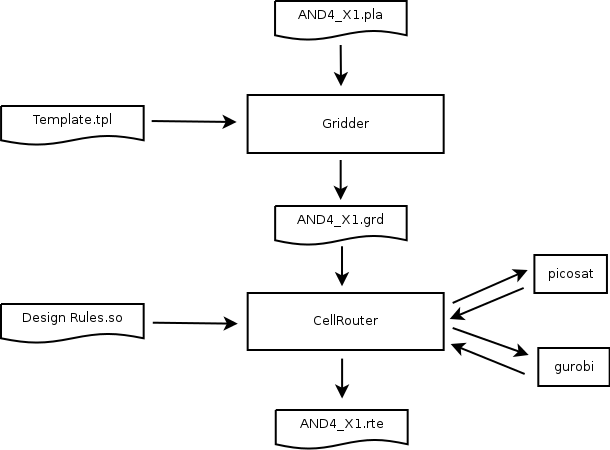
\includegraphics[scale=0.6]{img/design/basicflow.png}
  \caption{CellRouter data flow}
  \label{fig:basicflow}
\end{figure} 

The input to the flow is a $.pla$ file which contains a linear placement of the nets that must be routed. It is given to the $Gridder$, which is a C++ binary that, with the placement and a $.tpl$ template file, outputs a $.grd$, a grid containing the placed nets. The template file contains information related to the geometrical structure of the problem, for example the length of both $p$ and $n$ transistors on the cell. Figure \ref{fig:templates} shows five possible templates that a given netlist could be adapted to. In fact, the decision of which template to use is crucial, since a routing problem solvable for a template is not necessary solvable for another one. Figure \ref{fig:threetemplates} shows the result of gridding an AND gate using three different templates. The same placement is respected but the final grid may even vary on vertical height. \\


\begin{figure}[h!]
  \centering
  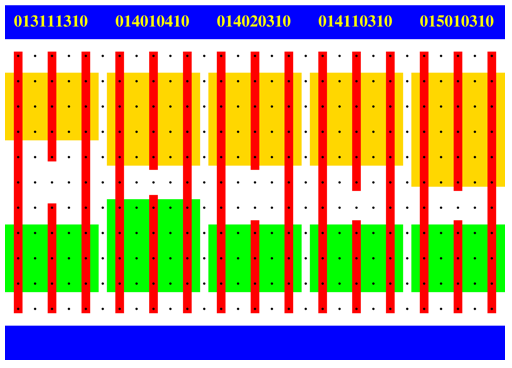
\includegraphics[scale=0.55]{img/design/templates.png}
  \caption{Five possible templates}
  \label{fig:templates}
\end{figure} 


\begin{figure}[h!]
  \centering
  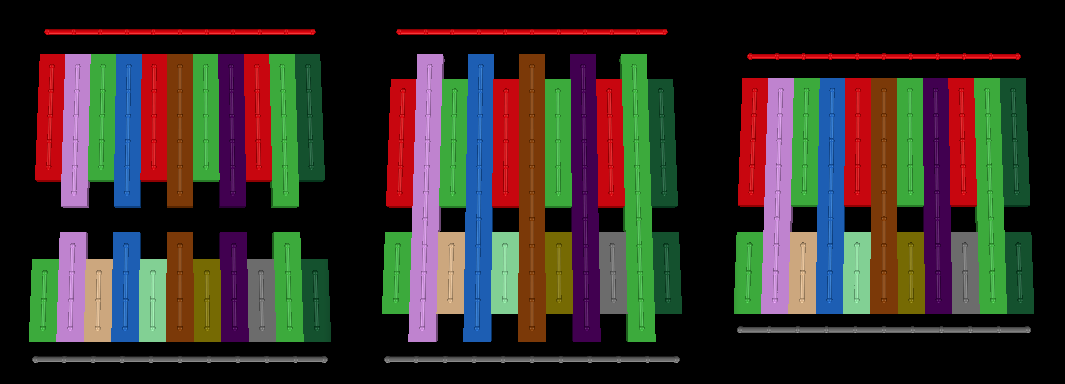
\includegraphics[scale=0.35]{img/design/threetemplates.png}
  \caption{Three different griddings for the same placement}
  \label{fig:threetemplates}
\end{figure} 

The resulting $.grd$ file represents the grid that will be routed by the CellRouter. More details about it can be found in appendix \ref{cha:gridformat}. CellRouter has been implemented in C++ and uses external software: \textit{picosat}, the SAT solver used to find the initial valid routing, and \textit{gurobi}, the mixed-integer linear programming tool used for optimization. Both processes are called internally from CellRouter when needed. In addition to the $.grd$, a file specifying the design rules to be followed by the router is required. It consists of a $.so$ library that is dynamically loaded, allowing different rule sets to be used for different routing  instances. Given such file and a $.grd$, CellRouter proceeds to find a valid assignment for the SAT formula and to optimize it using gurobi. More information on the interface of CellRouter can be found in appendix \ref{cha:cli}. \\

It is important to note that the problem of finding a routing for a given grid is a combinatorial optimization problem. The goal is to find the best possible grid in the set of those which are valid routings. The output of running CellRouter does not depend exclusively on the $.grd$ input and the specified design rules. A lot of parameters can be modified for CellRouter, either when looking for a solution or during optimization (halo size, number of escapes, heuristic rounds...). As we will see later, the use of divide-and-conquer techniques will make the  search space greater. This is a problem since the best configuration to route a given cell does not necessarily generate a good solution for another one. This inherent difficulty must be taken into account when designing the tool and the experiments. \\


\section{Design Decisions}

Given that the original tool was developed using C++, the first implementation that was made was a C++ binary called CellDivider. Its aim was to begin interacting with the problem, getting to know the data structures and overall flow. CellDivider received the same input that was before given to CellRouter and directly interacted with the infrastructure that called picosat and gurobi. It interacted directly with many of the classes that were used by the original tool. The grid data structure already existed in C++, so CellDivider focused on interacting with the problem through it. It did the most basic partition one could think of; given a cell as an input such as the one on Figure \ref{fig:C++buida}, the program generated a new cell that was exactly the left half of the original one (Figure \ref{fig:C++mitja}, left side). The router, called from inside CellDivider, solved the left-hand part (Figure \ref{fig:C++mitja}, right side). When solving a half of the problem, the program did not consider any information of the remainder of the cell. Finally, CellDivider copied the solution onto the original cell, as shown in Figure \ref{fig:C++plena}, and the partially routed problem was sent to the router to obtain a valid solution for the whole cell. \\

\begin{figure}[h!]
  \centering
  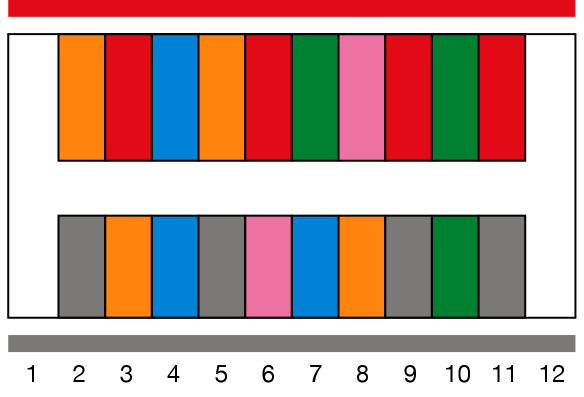
\includegraphics[scale=0.5]{img/design/CompletabuidaC++.png}
  \caption{Input for CellDivider}
  \label{fig:C++buida}
\end{figure} 

\begin{figure}[h!]
  \centering
  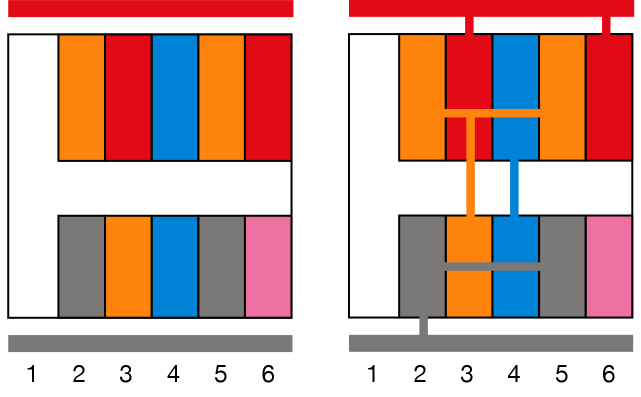
\includegraphics[scale=0.5]{img/design/MitjaC++.png}
  \caption{Partial problem and solution}
  \label{fig:C++mitja}
\end{figure} 

\begin{figure}[h!]
  \centering
  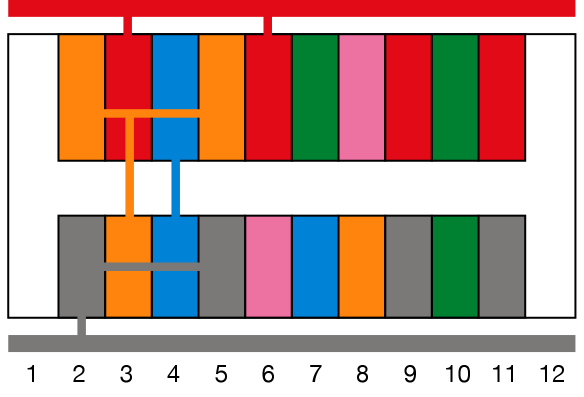
\includegraphics[scale=0.5]{img/design/CompletaplenaC++.png}
  \caption{Final routing problem}
  \label{fig:C++plena}
\end{figure} 


When the router receives a grid as an input all the variables are fixed, including those which come from an earlier partial solution. This first version showed how a poorly chosen distribution on a partial routing could lead the total cell to become unsatisfiable. It was tested against a subset of cells obtaining very different results, from cells that were unsatisfiable to cells that were routed in half the original time. From this moment on, the focus was set on obtaining partial solutions that were conscious of the rest of the cell, trying to avoid unsatisfiable global situations. \\

Following this first version, it was decided to use python to continue with the project and to leave CellRouter as it was, interacting with it through the command line and external files instead of modifying the router itself. The idea was to work at a grid level, separating CellDivider from the other parts of the project. Python seemed a good implementation language given that the work CellDivider itself does is not computationally intensive and that much prototyping and testing had to be done. Ipython was used to develop the project; it is a framework that allows using Python in a more interactive fashion, with improved debugging and an enriched web-based editor. \\

Given that CellDivider was going to be developed using python and work at a grid level, with the grid being a C++ data structure, SWIG was used to interface the class and use it from python. However, many problems arose when trying to create the interface for such a complex class and, finally, the grid data structure was replicated in python. Complete separation from the C++ project was achieved, so the development of CellDivider became independent of the internals of CellRouter. This involved some extra work as the original data structures were modified halfway through the project, which would have been easier if python accessed the C++ classes directly. \\

The final flow using CellDivider is shown in Figure \ref{fig:pythonflow}. CellDivider reads the cell.grd file, containing the grid to be routed, and a configuration file, which includes the routes of the cells, binaries and the design rules file. Several smaller grid routing problems are created. For each one, CellDivider creates a temp.grd file and writes in it the grid that needs to be routed. Then a CellRouter process is created, which uses temp.grd as an input and routes it independently. When the router ends, the routed grid is saved in a temp.rte file and CellRouter returns the output to CellDivider, including information such as if the cell was routable or not, computation time and other metrics. Finally, CellDivider creates a cell.rte file where the final routed cell is saved if a routing has been found, or announces the opposite otherwise. \\

\begin{figure}[h!]
  \centering
  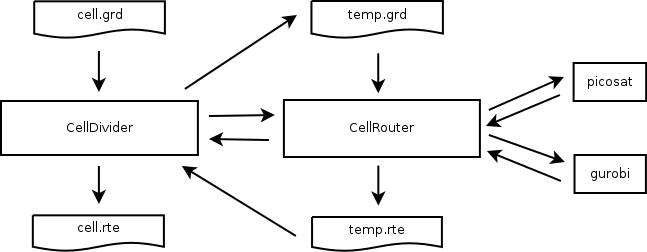
\includegraphics[scale=0.6]{img/design/pythonflow.png}
  \caption{CellDivider data flow}
  \label{fig:pythonflow}
\end{figure} 


\section{Conclusions}
In this chapter we have exposed what the design decisions have been for the development of the divide-and-conquer strategy, including the reasons why python was chosen as a development tool and how the contributions of this project adapt to the already existing framework. Many versions of CellDivider have existed due to the experimental nature of the problem. All of them share the basic functions, which include reading the configuration file, routing a set of cells specified on a given file and calling the Gridder, Cellrouter or Viewer, extracting information from their results. Aside from this common features, every version of CellDivider can be described in terms of their partition algorithm, how to prepare a partial routing, and their meta-algorithm, how to use the partial problems to obtain a global solution. The main task during the project has been coming up with several algorithms for both cases, as will be explained in next chapter.  \\


